% Figure 1: overview of the approach. Compiled by fig_pipeline.py; 16 cm wide, the text width of the manuscript.
\documentclass[border=1pt]{standalone}
% Shared preamble of the TikZ figures (fig_pipeline.tex, graphical_abstract.tex): the fonts and colors of the
% matplotlib figures (DejaVu Sans, palette of figures.py) and the arrow styles.
\usepackage[T1]{fontenc}
\usepackage{DejaVuSans}
\usepackage{DejaVuSansMono}
\renewcommand*\familydefault{\sfdefault}
\usepackage{xcolor}
\usepackage{tikz}
\usetikzlibrary{arrows.meta,calc}

\definecolor{ink}{HTML}{0B0B0B}
\definecolor{ink2}{HTML}{52514E}
\definecolor{boxedge}{HTML}{7D7C78}
\definecolor{boxfill}{HTML}{F4F3F0}
\definecolor{accent}{HTML}{2A78D6}
\definecolor{accentfill}{HTML}{E8F1FC}
\definecolor{bar}{HTML}{9A9994}
\definecolor{ngram}{HTML}{EB6834}

\tikzset{
  box/.style={draw=boxedge, fill=boxfill, rounded corners=3pt, line width=0.7pt, inner sep=0.12cm,
              anchor=north west},
  accentbox/.style={box, draw=accent, fill=accentfill},
  flow/.style={draw=ink2, line width=0.8pt, -{Stealth[length=5pt, width=4.5pt]}},
  line/.style={draw=ink2, line width=0.8pt},
  link/.style={flow, dash pattern=on 3pt off 2pt},
}
% small arrow for running text, e.g. "genome \arr{} loop pair"
\newcommand{\arr}{\tikz[baseline=-0.55ex]\draw[ink2, line width=0.5pt, -{Stealth[length=3.2pt, width=3pt]}]
  (0,0) -- (0.3,0);}


\newlength{\bw}\setlength{\bw}{3.28cm}      % text width of a box; outer width 3.52 cm
% box content: bold title, then the lines of #2 (separated by \\), top-aligned in a box of fixed height
\newcommand{\content}[2]{\begin{minipage}[t][1.62cm][t]{\bw}\centering
  {\fontsize{8.2}{10}\selectfont\bfseries\color{ink}#1\par}\vspace{3pt}
  {\fontsize{7.5}{9.2}\selectfont\color{ink2}#2\par}\end{minipage}}
\tikzset{note/.style={font=\fontsize{7.5}{9}\selectfont\itshape, text=ink2}}

\begin{document}
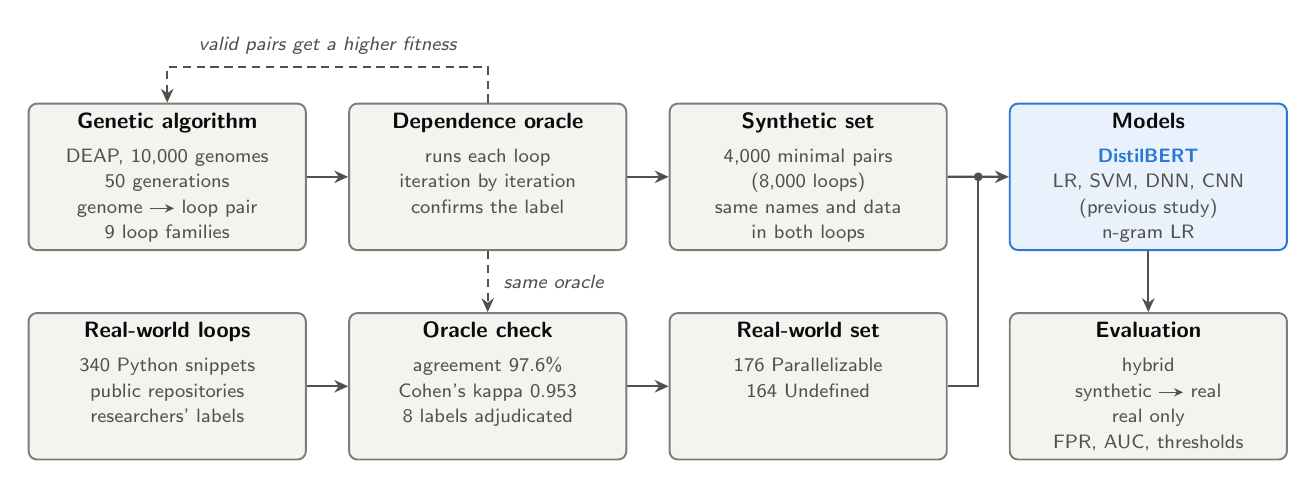
\begin{tikzpicture}
  % columns start at 0, 4.07, 8.14 and 12.46 cm; rows at 0 and -2.66 cm
  \node[box] (ga) at (0, 0) {\content{Genetic algorithm}{DEAP, 10,000 genomes\\50 generations\\
    genome \arr{} loop pair\\9 loop families}};
  \node[box] (oracle) at (4.07, 0) {\content{Dependence oracle}{runs each loop\\iteration by iteration\\
    confirms the label}};
  \node[box] (syn) at (8.14, 0) {\content{Synthetic set}{4,000 minimal pairs\\(8,000 loops)\\
    same names and data\\in both loops}};
  \node[accentbox] (models) at (12.46, 0) {\content{Models}{\textcolor{accent}{\bfseries DistilBERT}\\LR, SVM, DNN, CNN\\(previous study)\\
    n-gram LR}};

  \node[box] (real) at (0, -2.66) {\content{Real-world loops}{340 Python snippets\\public repositories\\
    researchers' labels}};
  \node[box] (check) at (4.07, -2.66) {\content{Oracle check}{agreement 97.6\%\\Cohen's kappa 0.953\\
    8 labels adjudicated}};
  \node[box] (realset) at (8.14, -2.66) {\content{Real-world set}{176 Parallelizable\\164 Undefined}};
  \node[box] (eval) at (12.46, -2.66) {\content{Evaluation}{hybrid\\synthetic \arr{} real\\real only\\
    FPR, AUC, thresholds}};

  % data flow
  \draw[flow] (ga) -- (oracle);
  \draw[flow] (oracle) -- (syn);
  \draw[flow] (real) -- (check);
  \draw[flow] (check) -- (realset);
  \coordinate (join) at ($(syn.east)!0.5!(models.west)$);
  \draw[line] (syn.east) -- (join);
  \draw[line] (realset.east) -| (join);
  \fill[ink2] (join) circle (1.6pt);
  \draw[flow] (join) -- (models.west);
  \draw[flow] (models) -- (eval);

  % the oracle verdict enters the fitness; the same oracle checks the real-world labels
  \draw[link] (oracle.north) -- ++(0, 0.45) -| node[pos=0.25, above=1pt, note] {valid pairs get a higher fitness}
    (ga.north);
  \draw[link] (oracle) -- node[right=2pt, note] {same oracle} (check);
\end{tikzpicture}
\end{document}
